\documentclass[twoside,privacy]{textmf-local/srathesis}
% options:
% [earlydraft] - Settings for quick draft printouts
% [germanthesis] - Thesis is written in German
% [plainunnumbered] - Don't print numbers on plain pages
% [privacy] - Generate a more privacy aware PDF (exclude birthplace and birthday)
% [twoside] - double sided
% [watermark] - Print current time/date at bottom of each page

% You can use dataref to reference data points from your experiments symbolical.
% Thereby, you are able to redo experiments, without reinserting and recalculating all numbers.
\usepackage{dataref}
\usepackage{pgfplots}
\renewcommand{\baselinestretch}{1.25}
\usepackage{xcolor}
\usepackage{tcolorbox}
\usepackage{multicol}
\definecolor{ba-green}{HTML}{008000}
\definecolor{ba-red}{HTML}{dc143c}

\definecolor{light-gray}{gray}{0.95}
\newcommand{\code}[1]{\colorbox{light-gray}{\texttt{#1}}}
% \input{data/dref}

\bibliography{references}
% The OSG also has a central bibliography that we share with the System- and Rechnerarchitecture (SRA) group from Hannover.
%\bibliography{bib/sra-ext}
%\bibliography{bib/sra-own}
%\bibliography{bib/osg-own}

\author{Elias Frank}
\title{Integration of reUpNix System and Container Updates with Azure IoT Edge and Docker}
\thesistype{Bachelorarbeit im Informatik}
\thesiscite{Bachelor's Thesis}
\birthday{15. Juni 1999}
\birthplace{Hamburg}
\thesisstart{11. Dezember 2023}
\thesisend{02. April 2024}
\examiner{Prof. Dr.-Ing. Christian Dietrich}
\coexaminer{Niklas Gollenstede (M.Sc.)}
\advisors{& \textbf{Niklas Gollenstede (M.Sc.)}}

\begin{document}

\pagestyle{fancy}
\pagenumbering{roman}

\maketitle

\chapter*{Abstract}
\addcontentsline{toc}{chapter}{Abstract}
% \begin{otherlanguage*}{american}

The growth of the \ac{IoT} in industries like production, manufacturing, and
agriculture has led to a wide range of innovations and new products. Currently
all major cloud providers such as Microsoft, Google, Amazon's AWS and IBM offer
\ac{IoT} services and solutions to their customers. However many \ac{IIoT} devices
which are installed in remote locations, such as offshore oil rigs or airplanes,
have limited, unstable, or costly network connections. Techniques to
minimize the \ac{IIoT} software’s network traffic both in message size
(such as \textit{Protobuf} or other forms of compression), and in message amount
(such as local processing with edge computing) have already been established.
However the image size, update, and consistency of the underlying operating
system is still a challenge. With Microsoft's \textit{Azure IoT Device
Update} service for example, the entire image for the operating system is sent
to the device and then written to a secondary partition. This results in hundreds
of megabytes being transmitted.

In this field study, we investigate if the \textit{NixOS}-based \textit{ReUpNix}
can be used as a suitable host operating system for Microsoft’s commercial
\ac{IoT} platform \textit{Azure IoT Edge}, since its image size is significantly
smaller than Microsoft's recommended Linux images.
Further, we investigate the conceptual advantages for \ac{IoT}
devices that \textit{NixOS}-based systems provide over traditional \textit{Linux}
operating systems, when updating the system. For this, we identified the
minimum set of components and features that have to be added to heavily minified
\textit{ReUpNix} in order to have the required functionality for the
Docker-container-based \textit{Azure IoT Edge}, while remaining at a small
footprint in disk size.

\textbf{[Expected result]}
With \textit{ReUpNix} as a host operating system for \textit{Azure IoT Edge}, we
observed A\% smaller image size due to the minification and B\% smaller size of
system updates due to the fact that only differences are sent, compared to
Microsoft's recommended \textit{Ubuntu 22.04} and a custom \textit{Yocto Linux}
image. Further we showed that it is possible to pre-install Docker container
layers on the device, such that the amount of data that needs to be transmitted
in the case of a container update with \textit{Azure IoT Edge} is heavily reduced.
However \textit{NixOS}-based systems do not receive official support from
Microsoft and product managers need to decide if the benefits outweigh the loss
of Microsoft's support.

% \end{otherlanguage*}


%\chapter*{Kurzfassung}
%\addcontentsline{toc}{chapter}{Kurzfassung}
%\begin{otherlanguage*}{ngerman}

%Gleicher Text in Deutsch

% \end{otherlanguage*}

\acresetall

\cleardoublepage
\tableofcontents

\cleardoublepage
\pagenumbering{arabic}


\chapter{Introduction}
\chapter{Introduction}
%\chapter{Einleitung}
\label{sec:introduction}

\begin{tcolorbox}[title=TODO]
general motivation for your work, context and goals: 1-2 pages

\begin{itemize}
\item \textbf{Context:} make sure to link where your work fits in
\item \textbf{Problem:} gap in knowledge, too expensive, too slow, a deficiency, superseded technology
\item \textbf{Strategy:} the way you will address the problem
\end{itemize}
\end{tcolorbox}

\section{Context}
\section{Problem}
\section{Strategy}


\chapter{Fundamentals}
This chapter introduces the major concepts, technologies,
and software relevant to this thesis. First, it will introduce the operating
systems \textit{Ubuntu 22.04}, \textit{Yocto Kirkstone Linux}, \textit{NixOS},
and \textit{ReUpNix}, which will be used for comparison in the later experiments.
Further, the \textit{Azure IoT Edge} platform by Microsoft will be introduced
with all the components that are used.
Finally, the last subsections will give an overview of the related work.

\section{Ubuntu 22.04}
\textit{Ubuntu 22.04} is the latest long-term support release of the
\textit{Linux}-based operating system \textit{Ubuntu} developed by Canonical.
It will receive updates and support for the next 5 years, until April
2027 \cite{ubuntu-releasenote}. Additionally, it is one of Microsoft's
recommended operating systems to run containerized applications with
\textit{Azure IoT Edge} on Linux \cite{msdoc-supportetplatforms}. For all the
tests and comparisons in this thesis, an \textit{Ubuntu 22.04} image was prepared
with \textit{Docker}, \textit{Azure IoT Edge} and \textit{Azure Device Update Agent}
installed, in addition to the default packages that come with the image. Like
with most \textit{Debian}-based systems, \textit{Ubuntu} uses the \textit{apt-get}
package manager by default to install, update, and remove software packages \cite{book:344012}.
However, when managing a fleet of \ac{IoT} devices, the update process can be
centralized with the \textit{Azure IoT Device Update Service} (see subsection
\ref{sec:azure-iot-device-update-service}) and applied with an A/B partitioning scheme.

\section{Yocto Kirkstone Linux}
The \textit{Yocto Project} is an open-source collaboration project that provides tools
and resources for building custom Linux-based systems for embedded devices.
\textit{Yocto Kirkstone Linux} is a recent long-term support release of the
\textit{Yocto Project}, which will receive support until April 2026 \cite{yocto-releases}.
The \textit{Yoctc Kirkstone} image, used for comparison in this thesis, was built
with the \textit{Yocto Project} tools and the \textit{meta-azure-iot-edge} layer.
Additionally, the image also contains \textit{Docker}, \textit{Azure Device Update Agent}
and common packages that are typically found on \textit{Linux} systems like \ac{SSH}
and \textit{systemd}.


\section{NixOS}
\textit{NixOS} is a \textit{Linux}-based operating system that uses the purely
functional package manager \textit{Nix}. It is currently maintained as
an open source project by the non-profit organization \textit{NixOS Foundation}
and the \textit{NixOS Community}. The project was started in 2003 by Eelco Dolstra,
who is the current president of the \textit{NixOS Foundation} as
a research project at the Utrecht University \cite{dolstra2003} and was introduced
as \textit{NixOS} in his 2008 paper "NixOS: A Purely Functional Linux Distribution"
\cite{dolstra2008}.

A \textit{NixOS} system is configured with a set of configuration files, which
are evaluated by the \textit{Nix} package manager to produce a complete system.
The configuration files are written in the functional \textit{Nix} programming language,
which has the advantage of being declarative and reproducible. Further, \textit{Nix}
utilizes cryptographic hashes to verify the integrity of the inputs and outputs
for any given build. This means that the same configuration inputs produce the
same system and it ensures the integrity of the entire system. This approach
aims to improve the correctness and reliability of
system deployments over traditional system build tools \cite{dolstra2006}.

A key concept of \textit{NixOS} is the \textit{Nix Store}, where all packages,
files, configurations, and other artifacts that the system requires are stored.
The \textit{Nix Store} is an immutable directory tree, where every \textit{Nix Store}
object is uniquely identified by its content hash and additionally a
human-readable name and version. In contrast to other operating systems where the package
manager is only used to manage the installation and removal of packages, in \textit{NixOS}
it is also used to manage the system configuration (typically stored in the
\textit{/etc} directory) and other static parts of the
system \cite{1411255}.

Lastly, \textit{NixOS} provides the option to perform a rollback of the system to a
previous configuration. \textit{NixOS} will keep the previous configuration
in a list of generations for this purpose \cite{1411255}, allowing users to easily
revert to a known stable state in case of errors or undesired changes. This
feature provides an efficient way to manage system updates and changes over time.

\section{ReUpNix}
\textit{reUpNix} is a research project at the Hamburg University of Technology,
which aims to improve the shortcomings of \textit{NixOS} specifically for
embedded and \ac{IoT} devices. It was introduced at the International Conference on
\ac{LCTES} in 2023 and is primarily maintained by Niklas Gollenstede.

Since \textit{NixOS} is a general-purpose operating system, it is not optimized
for embedded and \ac{IoT} devices. As a result of this, the base image size of
\textit{NixOS} is relatively large since it aims to support a wide range of
software and hardware for different use cases. \textit{reUpNix} aims to address
this issue by providing a minification process, which removes unnecessary
files, configurations, and applications from the base image \cite{gollenstede:23:lctes}.

Additionally, it addresses the problem of the update size, which is an important
factor for \ac{IoT} devices, since they might have limited bandwidth and
potentially unreliable connections. The regular update mechanism for \textit{Nix}
will compute which dependencies are required and are not already present in the \textit{Nix Store}.
Once the dependencies are computed, the required packages are downloaded and
placed in the \textit{Nix Store}, regardless of how many files were changed inside
the package. In a desktop or server environment, this
update process is typically not an issue, since these devices are usually
connected via high-speed internet connections. In contrast, an \ac{IoT} device
would waste a lot of bandwidth and time to download packages in which only a
small set of files have changed. \textit{reUpNix} addresses this issue by
replacing the regular \textit{Nix} update mechanism with a custom update mechanism
that only downloads the difference and applies them to the \textit{Nix Store}
\cite{gollenstede:23:lctes}.

Finally, \textit{reUpNix} provides a way to declaratively define and update
the configuration for the bootloader as well as disk partitioning. This wasn't
covered by \textit{NixOS} before and is a crucial feature for embedded and
\ac{IoT} devices \cite{gollenstede:23:lctes}.

\section{Azure IoT}
\textit{Azure IoT} is a cloud platform provided by Microsoft that
empowers organizations to build, deploy, and manage \ac{IoT} solutions at scale.
\textit{Azure IoT} offers a suite of services and tools designed to connect,
monitor, and control a diverse array of devices, sensors, and equipment. The
platform enables integration of \ac{IoT} devices with Microsoft's other cloud
services, facilitating the collection and analysis of data for actionable insights.
The \ac{IoT} platform supports a wide range of industries and uses cases,
for customers to build their own \ac{IoT} solutions \cite{msdoc-aziot}.

While the "big three" cloud service providers, namely Microsoft, Amazon and
Google, all offer \ac{IoT} platforms and services, a conducted comparison finds
that Microsoft's \textit{Azure IoT} provides the most tools for businesses,
especially data visualization tools. Hover, Amazon's \textit{AWS} \ac{IoT}
offerings have the largest market share \cite{9116254}.

\subsection{Azure IoT Identity Service}
The \textit{Azure IoT Identity Service} is a set of system services developed
by Microsoft that \ac{IoT} developers can leverage to build applications that
communicate with the \textit{Azure IoT} cloud platform. They provide abstractions
for provisioning, managing, and authenticating devices, as well as managing
certificates and secrets on the device \cite{aiiot}. The services are implemented
in the Rust programming language and run under Linux-based systems as \textit{systemd}
services.


\subsection{Azure IoT Edge}
The \textit{Azure IoT Edge} platform is a collection of software products and
services developed and maintained by Microsoft that extends the capabilities
of \textit{Azure IoT} to the edge of the network. This platform facilitates the
deployment and management of \ac{IoT} devices, enabling them to run \ac{AI},
machine learning, and analytics locally. Azure IoT Edge allows organizations to
process and analyze data on-site, near the data source, reducing latency and
optimizing bandwidth usage.
Unlike traditional cloud computing, where data is sent to a centralized server
for analysis, edge computing occurs on or near the device or "edge" of the
network. This approach is particularly valuable in scenarios where quick
response times are critical or where excessive data transfer to the cloud
is not possible \cite{msdoc-aziotedge}.

All software, as well as \ac{SDK}s and
libraries, which are installed on the device, are open source. Hover, the
cloud services offered by Microsoft are almost exclusively closed source.
Development and maintenance of \textit{Azure IoT Edge} is publicly visible on
\textit{GitHub}. The biggest contributions
to the public repository are made by Microsoft employees Varun Puranik,
Philip Lin and Damon Barry, but it also features bug-fixes and contributions
from the community and non-Microsoft employees
\footnote{Full overview of all contributions: https://github.com/Azure/iotedge/graphs/contributors}.


\subsection{Azure IoT Edge Agent}
In Microsoft's terminology, containerized workloads, which will be run on the \ac{IIoT}
devices, are called \textit{IoT Edge Modules}.
The \textit{Azure IoT Edge Agent} is a crucial component of the \textit{Azure IoT Edge}
platform, responsible for managing the lifecycle of \textit{IoT Edge Modules} and
handling communication between these modules and the \textit{Azure IoT Hub}.
It executes the deployment, configuration, and monitoring of modules running on
edge devices by communicating with the \ac{OCI}-container runtime,
ensuring that they function according to defined deployment and settings.
The \textit{Azure IoT Edge Agent} also leverages the \textit{Azure IoT Identity Service}
for secure communication, handling authentication and encryption for data exchange
between the edge devices and the cloud \cite{msdoc-aziotedge-arch}.


\subsection{Azure IoT Hub}
The \textit{Azure IoT Hub} is a cloud service developed by Microsoft, designed to
enable secure and scalable communication between a fleet of \ac{IoT} devices and
the cloud. It serves as a central message queue, enabling devices to send telemetry
data, and be managed remotely. By default, the devices communicate with the
\textit{Azure IoT Hub}
via the \ac{AMQP} protocol, which is a lightweight, reliable, and efficient
messaging protocol and can route the received messages to other cloud services,
including services by Microsoft, such as \textit{Azure Stream Analytics} or
\textit{Azure Data Explorer}.
With features such as device registration,
authentication, and monitoring, the \textit{Azure IoT Hub} provides a reliable and efficient
way to connect and manage a diverse fleet of \ac{IoT} devices, with which
organizations and developers can build and deploy \ac{IoT} solutions at scale \cite{msdoc-aziothub}.

\subsection{Azure IoT Device Update Service}
\label{sec:azure-iot-device-update-service}
The \textit{Azure IoT Device Update Service} is a cloud service by Microsoft
for managing and automating the firmware and system updates of \ac{IoT} devices at scale.
It enables organizations to securely deploy, monitor, and schedule updates for
a large number of connected devices, ensuring they are always up-to-date with
the latest security patches, bug fixes, and feature enhancements. This service
simplifies the management of device updates, offering capabilities such as
rollback options, group-based deployments, and detailed reporting to track the
status of updates across diverse \ac{IoT} device fleets. In order to use the service,
the devices must be running the \textit{Azure IoT Edge} runtime, as well as the
\textit{Azure IoT Device Update Agent}, a \textit{systemd} service which is
responsible for the communication with the \textit{Azure IoT Device Update Service}
\cite{msdoc-adu}. Device update images can be uploaded to the
\textit{Azure IoT Device Update Service} with a specific update manifest, in
which all the necessary information about the update is specified, such as the
version and target devices. Once an update is triggered, the \textit{Azure IoT Device Update
Agent} will download the updated image and apply it to the device and depending
on the specified format will either perform an update in an A/B partitioning
schema or will run a custom update script.


% \section{Related Work}


\chapter{Architecture}
\chapter{Architecture}

Developed architecture / system design / implementation: 1/3

\begin{itemize}
\item start with a theoretical approach
\item describe the developed system/algorithm/method from a high-level point of view
\item go ahead in presenting your developments in more detail
\end{itemize}

\section{Sample Application}
For verifying that the \textit{Azure IoT Edge} software behaves correctly
with the given operating system, a sample application was developed. This
containerized sample application sends a randomly generated number to the
\textit{Edge Hub}.

The application features a \ac{HTTP} \ac{REST} \ac{API} for further automation.

\begin{table}[H]
    \centering
    \begin{tabular}{ p{0.33\textwidth} p{0.14\textwidth} p{0.45\textwidth}}
        \toprule
        \textbf{Container Name} & \textbf{Developer} & \textbf{Description} \\
        \midrule
        Edge Agent & Microsoft & Application for managing containers and deployments. \\
        Edge Hub & Microsoft & Gateway and buffer for sending messages to cloud services. \\
        Edge Metrics Collector & Microsoft & Application for collecting container logs, metrics and health data. \\
        SQL Server & Microsoft & Containerized instance of Microsoft's SQL server. \\
        sampleapp UI & Elias Frank & Web application for viewing telemetry data from the \ac{API}. \\
        sampleapp API & Elias Frank & \ac{REST} \ac{API} for retrieving telemetry locally for further automation. \\
        sampleapp Telemetry Service & Elias Frank & Background service for randomly generating telemetry. \\
        \bottomrule
    \end{tabular}
    \caption{Sample Application: List of containers}
\end{table}

\begin{table}[H]
    \centering
    \begin{tabular}{l l l l }
        \toprule
        \textbf{From} & \textbf{To} & \textbf{Port} & \textbf{Protocol} \\
        \midrule
        sampleapp Telemetry Service & Edge Hub & C & D \\
        sampleapp Telemetry Service & SQL Server & C & D \\
        Edge Metrics Collector & Edge Agent & 9000 & \ac{HTTP} \\
        Edge Metrics Collector & Edge Hub & 9000 & \ac{HTTP} \\
        Edge Metrics Collector & sampleapp API & 8080 & \ac{HTTP} \\
        Edge Metrics Collector & sampleapp Telemetry Service & 8080 & \ac{HTTP} \\
        \bottomrule
    \end{tabular}
    \caption{Sample Application: Communication table}
\end{table}


\begin{figure}[H]
    \includegraphics[width=\textwidth]{fig/sample-app-dataflow.drawio.png}
    \caption{Sample Application: Architecture Overview}
    \label{fig:sample-app-architecture}
\end{figure}

\section{Experiments}
\subsection{Image size}
When updating the operating system with an A/B failover model, the entire
image needs to be downloaded and written to a secondary partition. In this
\ac{OTA} scenario the size of the operating system image is critical.
For this experiment two sizes are relevant, when comparing operating systems.
Firstly, the actual size of the image that needs to be written to the partition.
Secondly, the size that the entire system takes up on the disk after booting.
\subsubsection{Transmitted image size}
\subsubsection{Size on disk}
The size on disk will be measured after the system has successfully booted
and started all \textit{Azure IoT Edge} services including the containerized
applications. To see if the containers have been successfully started,
Microsoft provides the command line interface \textit{iotedge}.
With the following command, it is possible to list all running containers.\\

\begin{lstlisting}[caption=Command to retrieve the status of all containers]
iotedge list
\end{lstlisting}
After all containers are running, it is possible to read out the disk utilization
with the \textit{df} command line interface. \cite{man-df}\\

\begin{lstlisting}[caption=Command to report file system space usage]
df -h
\end{lstlisting}
The value of the disk utilization excluding the \textit{/var} directory
can be used for comparing operating systems.



\subsection{Time to recover}
\subsection{Endurance}

\chapter{Analysis}
\chapter{Analysis}

Measurement results / analysis / discussion: 1/3

\begin{itemize}
\item whatever you have done, you must comment it, compare it to other systems, evaluate it
\item usually, adequate graphs help to show the benefits of your approach
\item caution: each result/graph must be discussed! what's the reason for this peak or why have you ovserved this effect
\end{itemize}

\section{Transmitted image size}
\begin{figure}[H]
\centering
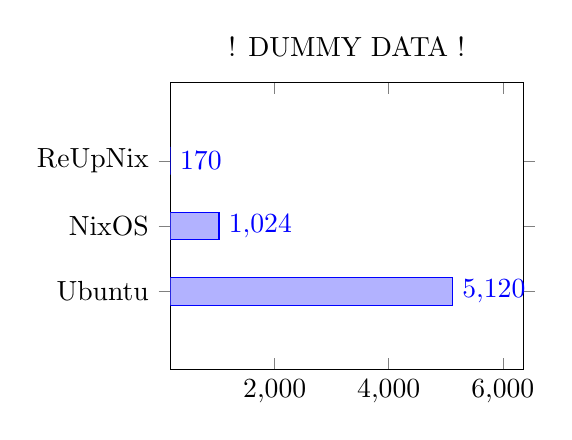
\begin{tikzpicture}
  \begin{axis}[
    title  = ! DUMMY DATA !,
    xbar,
    ytick             = data,
    enlarge y limits  = 0.6,
    enlarge x limits  = { 0.25, upper},
    width = 0.5\textwidth,
    symbolic y coords = {Ubuntu, NixOS, ReUpNix},
    nodes near coords,
  ]
  \addplot coordinates { (170,ReUpNix)         (1024,NixOS)
                         (5120,Ubuntu)   };
  \end{axis}
\end{tikzpicture}
\caption{Image size by OS in megabytes}
\end{figure}

\section{Disk usage}
\begin{figure}[H]
\centering
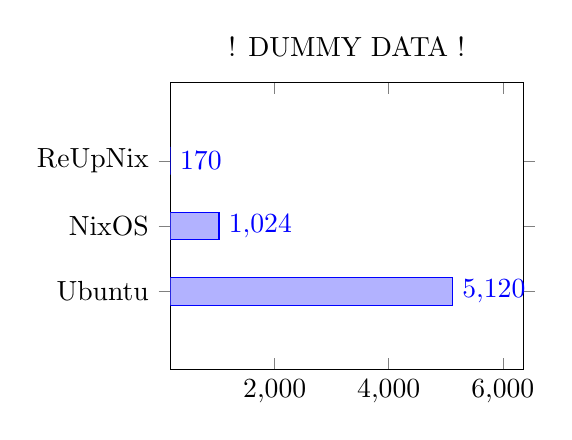
\begin{tikzpicture}
  \begin{axis}[
    title  = ! DUMMY DATA !,
    xbar,
    ytick             = data,
    enlarge y limits  = 0.6,
    enlarge x limits  = { 0.25, upper},
    width = 0.5\textwidth,
    symbolic y coords = {Ubuntu, NixOS, ReUpNix},
    nodes near coords,
  ]
  \addplot coordinates { (170,ReUpNix)         (1024,NixOS)
                         (5120,Ubuntu)   };
  \end{axis}
\end{tikzpicture}
\caption{Disk utilization after boot by OS in megabytes}
\end{figure}

\section{Mean time to recover}
\begin{figure}[H]
\centering
\begin{tikzpicture}
  \begin{axis}[
    title  = ReUpNix,
    ybar,
    enlarge y limits  = {0.15,upper},
    width = 0.5\textwidth,
    nodes near coords,
  ]
    \addplot table [x=seconds, y=times, col sep=comma] {data/time-to-recover-reupnix.csv};
  \end{axis}
\end{tikzpicture}
\begin{tikzpicture}
  \begin{axis}[
    title  = NixOS,
    ybar,
    enlarge y limits  = {0.15,upper},
    width = 0.5\textwidth,
    nodes near coords,
  ]
    \addplot table [x=seconds, y=times, col sep=comma] {data/time-to-recover-nixos.csv};
  \end{axis}
\end{tikzpicture}
\begin{tikzpicture}
  \begin{axis}[
    title  = Ubuntu 22.04,
    ybar,
    enlarge y limits  = {0.15,upper},
    width = 0.5\textwidth,
    nodes near coords,
  ]
    \addplot table [x=seconds, y=times, col sep=comma] {data/time-to-recover-ubuntu.csv};
  \end{axis}
\end{tikzpicture}
\caption{Time of recovery after a reboot by OS in seconds.}
\end{figure}

\chapter{Conclusion}
\section{Summary}
In this thesis we have investigated the possibility of using \textit{reUpNix} as the
host \ac{OS} for running the popular \textit{Azure IoT} platform on \ac{IIoT} devices.
We have focused on the update mechanism of \textit{reUpNix} and how it can be used
to save bandwidth when updating the \ac{OS} and \ac{OCI}-container images on the device,
since some \ac{IoT} devices have limited bandwidth because they are installed in
remote locations and/or have limited storage. We were able to show that \textit{Azure IoT Edge}
can be packaged and run on the \textit{Nix}-based \textit{reUpNix} and
\textit{reUpNix}'s \textit{Nix store} does not introduce any significant overhead
or delay when recovering from a reboot. When comparing \textit{reUpNix} to
other \ac{OS} that are able to run \textit{Azure IoT Edge}, we observed that \textit{reUpNix}
had a significantly smaller image size than the other \ac{OS}. In particular,
\textit{reUpNix} has a 43\% smaller image size than for example Microsoft's
recommended \textit{Ubuntu 22.04}. We also showed that \textit{reUpNix}'s update
methodology is significantly more efficient than the commonly used A/B partition
schema. In our tests, \textit{reUpNix} was able to update the \ac{OS} and save
90.3\% of the transferred data compared to a A/B partition schema with \textit{Ubuntu 22.04}.


\section{Conclusion}
It was shown that reUpNix has the the potential to drastically reduce the transferred
data when updating the operating system, which is important for \ac{IIoT} devices
that have a limited Internet connection. \textit{reUpNix} provides a viable
alternative for \ac{IoT} devices running \textit{Azure IoT Edge}
to the commonly used A/B partition schema, which is used by most platforms,
including the \textit{Azure Device Update Service}.

However, Microsoft does not officially support NixOS or reUpNix, which may be a decisive factor
for product managers choosing an \ac{OS} for their \ac{IIoT} devices. Microsoft
only provides so called "Tier 1" support for Ubuntu, Debian, Red Hat Enterprise
Linux and Windows, which means that Microsoft is actively testing and validating
new releases. If a developer is using an \ac{OS} that is not officially supported
and encounters a problem, they need to reproduce the issue with one of Microsoft's
"Tier 1" supported \ac{OS} before they can open a support ticket with Microsoft
\cite{msdoc-supportetplatforms}.

Lastly, \textit{reUpNix}'s differential updates also reduce the data transmitted
when updating or installing \ac{OCI}-container images, compared to using \code{docker pull}.
This is important for \ac{IIoT} devices that run \textit{Azure IoT Edge} or other
container runtimes, which enables them to update their container images more frequently
and bring customers new features faster in an edge computing environment.


\section{Future Work}
In order to store the \ac{OCI}-container images in the \textit{Nix store} and
handle the update of the images easier, we could implement a custom storage
provider for docker images that uses the \textit{Nix store} as the backend.
This would eliminate some of the complexity of the current solution and reduce
the overhead required to load the container images.

Further, we could investigate the possibility of implementing a custom update
handler for the \textit{Azure Device Update Agent} since Microsoft allows
the implementation of custom update handlers. This would allow us replace the
currently script handler with a dedicated update handler that is compatible
with \textit{reUpNix}'s update mechanism and has lower overhead.

Lastly, we have not shown that the system we have built is the smallest possible
system to run \textit{Azure IoT Edge} on. There are still possibilities to explore, which
further minify the system, such as using \textit{Podmand} instead of \textit{Docker}
or minifying the \textit{Azure IoT Edge} runtime and the \textit{Azure IoT Edge} modules
or using software like \textit{upx} to compress binaries.


\cleardoublepage

\pagestyle{fancy-lists}

% \phantomsection is needed for hyperref to reference the correct
% page.

\phantomsection
% special page style for the unnumbered lists chapter and its sections.  This
% prevents numbers in the headers.  The title is set via \chaptermark and
% \sectionmark, see below.
\addcontentsline{toc}{chapter}{\listoftitlename}%
\chaptermark{\listoftitlename}

\addcontentsline{toc}{section}{\glossarytitlename}%
\sectionmark{\glossarytitlename}
\chapter*{\glossarytitlename}
\chapter*{\glossarytitlename}

\begin{acronym}
\acro{WSN}{Wireless Sensor Network}
\acro{MANET}{Mobile Ad Hoc Network}
\acro{IoT}{Internet of Things}
\acro{IIoT}{Industrial IoT}
\acro{OCI}{Open Container Initiative}
\acro{SDK}{Software Development Kit}
\end{acronym}

\cleardoublepage

\phantomsection
\addcontentsline{toc}{section}{\listfigurename}%
\sectionmark{\listfigurename}
\listoffigures
\cleardoublepage

\phantomsection
\addcontentsline{toc}{section}{\listtablename}%
\sectionmark{\listtablename}
\listoftables
\cleardoublepage

\phantomsection
\addcontentsline{toc}{section}{\listlistingname}%
\sectionmark{\listlistingname}
\listoflistings
\cleardoublepage

% \phantomsection
% \addcontentsline{toc}{section}{\listalgorithmname}%
% \sectionmark{\listalgorithmname}
%\listofalgorithms
% \cleardoublepage

\phantomsection
\addcontentsline{toc}{section}{\bibname}%
\sectionmark{\bibname}
\printbibliography

\end{document}
